\documentclass[a4paper]{article}
\usepackage{amsmath,amssymb,algorithmic,booktabs,bm,caption,cases,csvsimple,enumerate,float,geometry,graphicx,indentfirst,listings,makecell,multirow,setspace,tabularx,titlesec,xcolor}
\captionsetup[figure]{labelsep=period}
\captionsetup[table]{labelsep=period}
\geometry{left=3.5cm,right=3.5cm,top=3.3cm,bottom=3.3cm}
\renewcommand\thesection{\arabic{section}}
\setlength{\parindent}{2em}
\begin{document}
\begin{center}
\huge
\textbf{VE216\\Introduction to Signals and Systems\\}
\Large
\vspace{30pt}
\uppercase{Prelab 2 Attached Pages}\\
\vspace{5pt}\today\\
\vspace{5pt}
Yihua Liu 518021910998
\vspace{5pt}
\rule[-10pt]{.97\linewidth}{0.05em}
\end{center}
\definecolor{mygray}{rgb}{0.9,0.9,0.9}
\lstset{
    language=Matlab,
    frame=shadowbox,
    numbers=left,
    breaklines=true,
    backgroundcolor=\color{mygray}
}

3.1 (b)
\begin{figure}[H]
    \begin{center}
        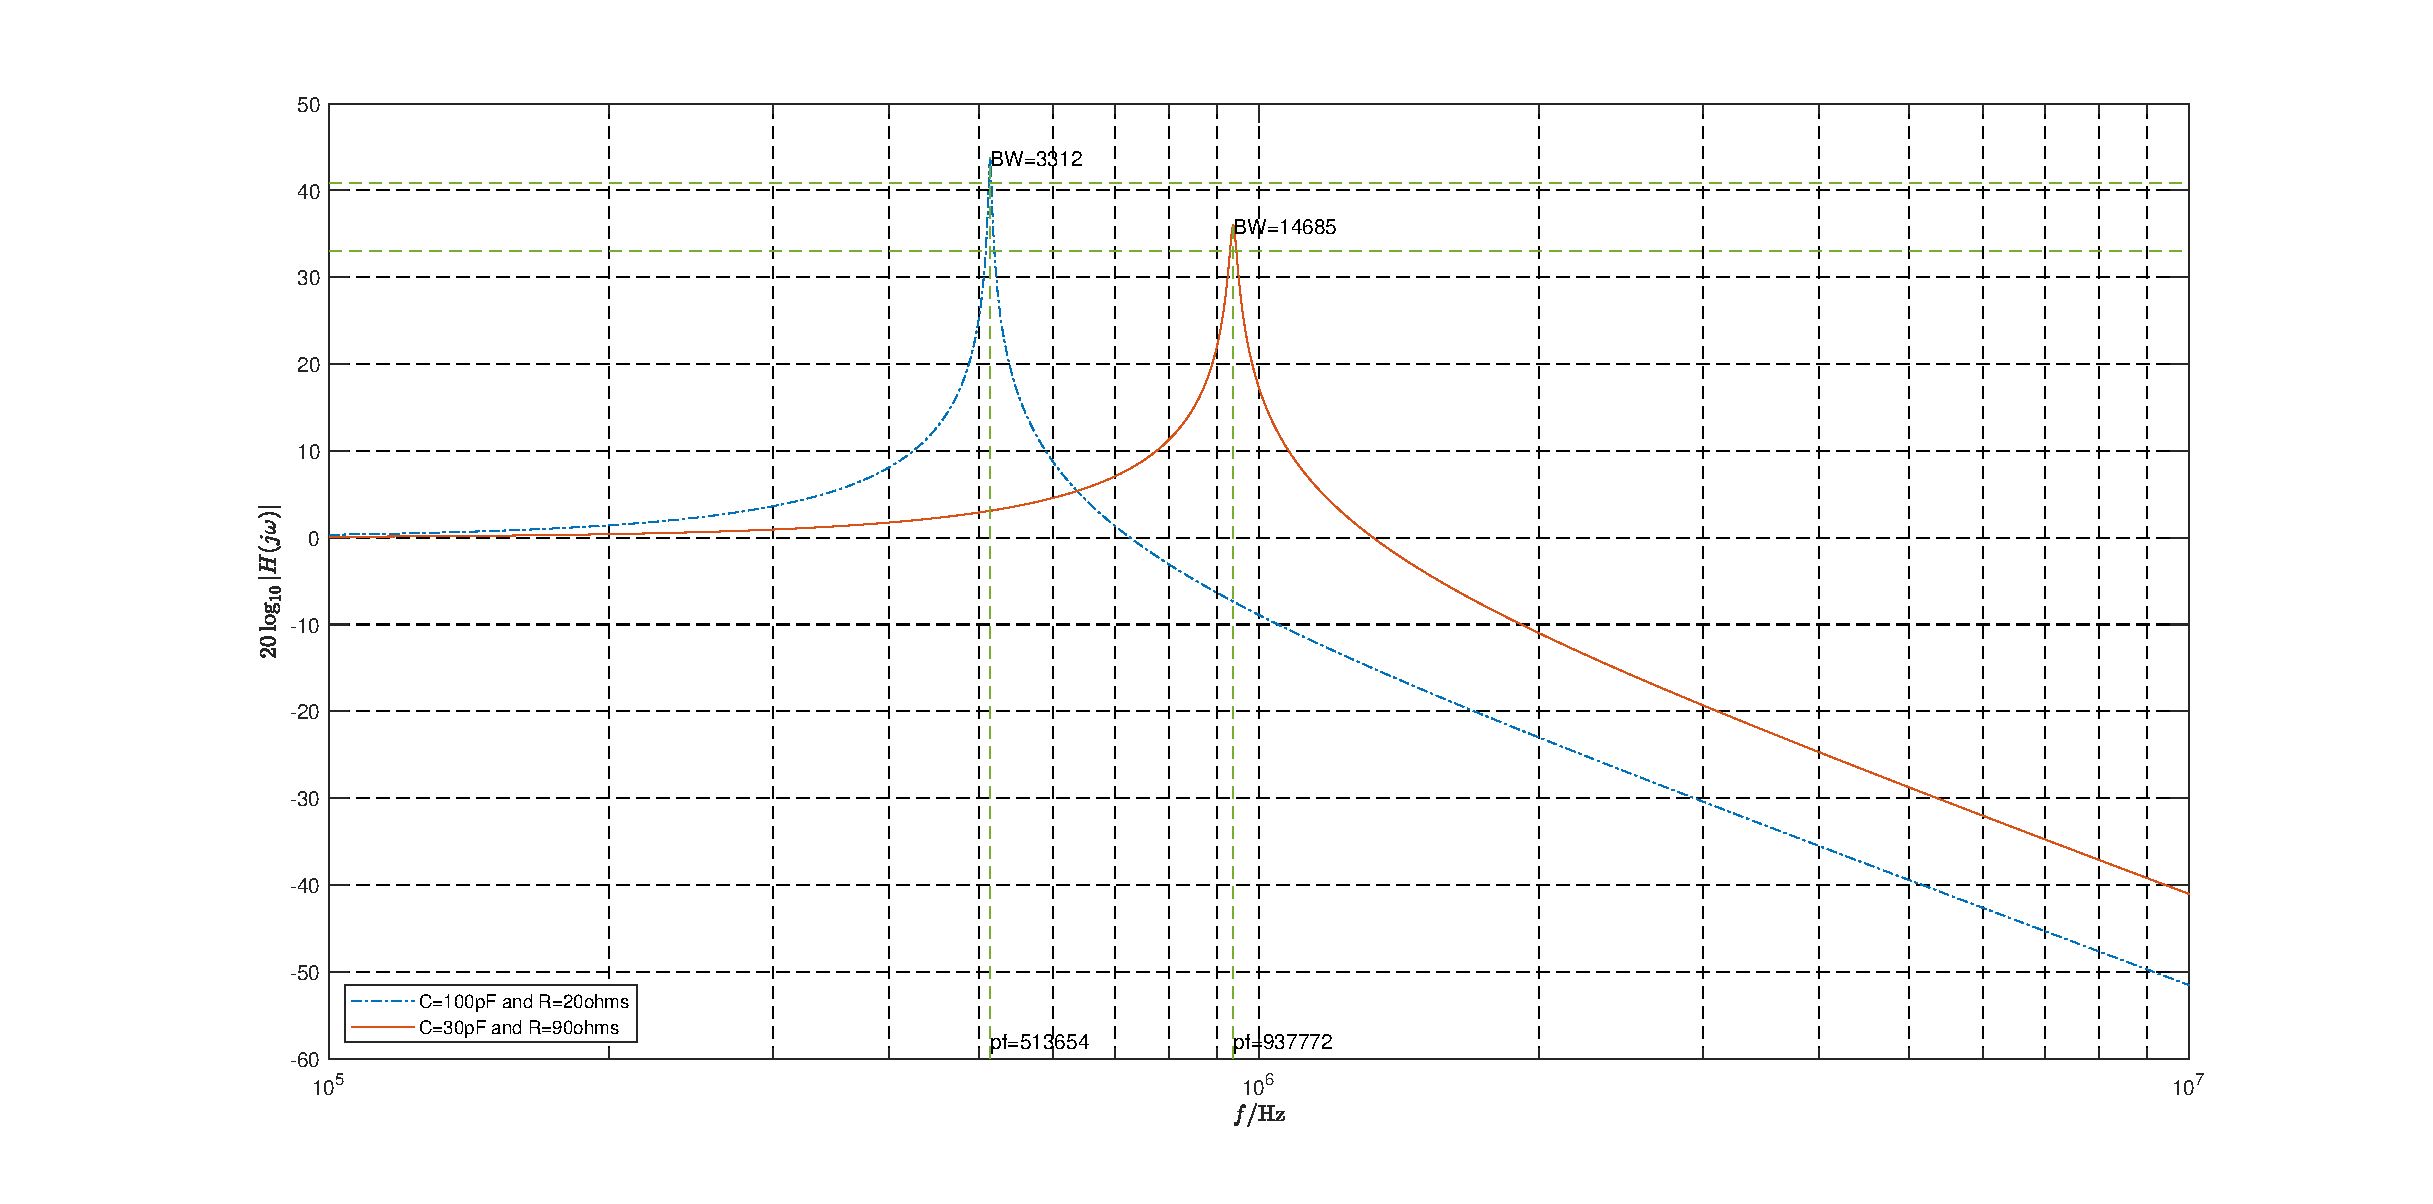
\includegraphics[width=1\textwidth]{3.1(b).eps}
    \end{center}
    \caption{3.1(b).}
\end{figure}
MATLAB Code:
\lstinputlisting{P3_1_b.m}

3.2 (c)
\begin{figure}[H]
    \begin{center}
        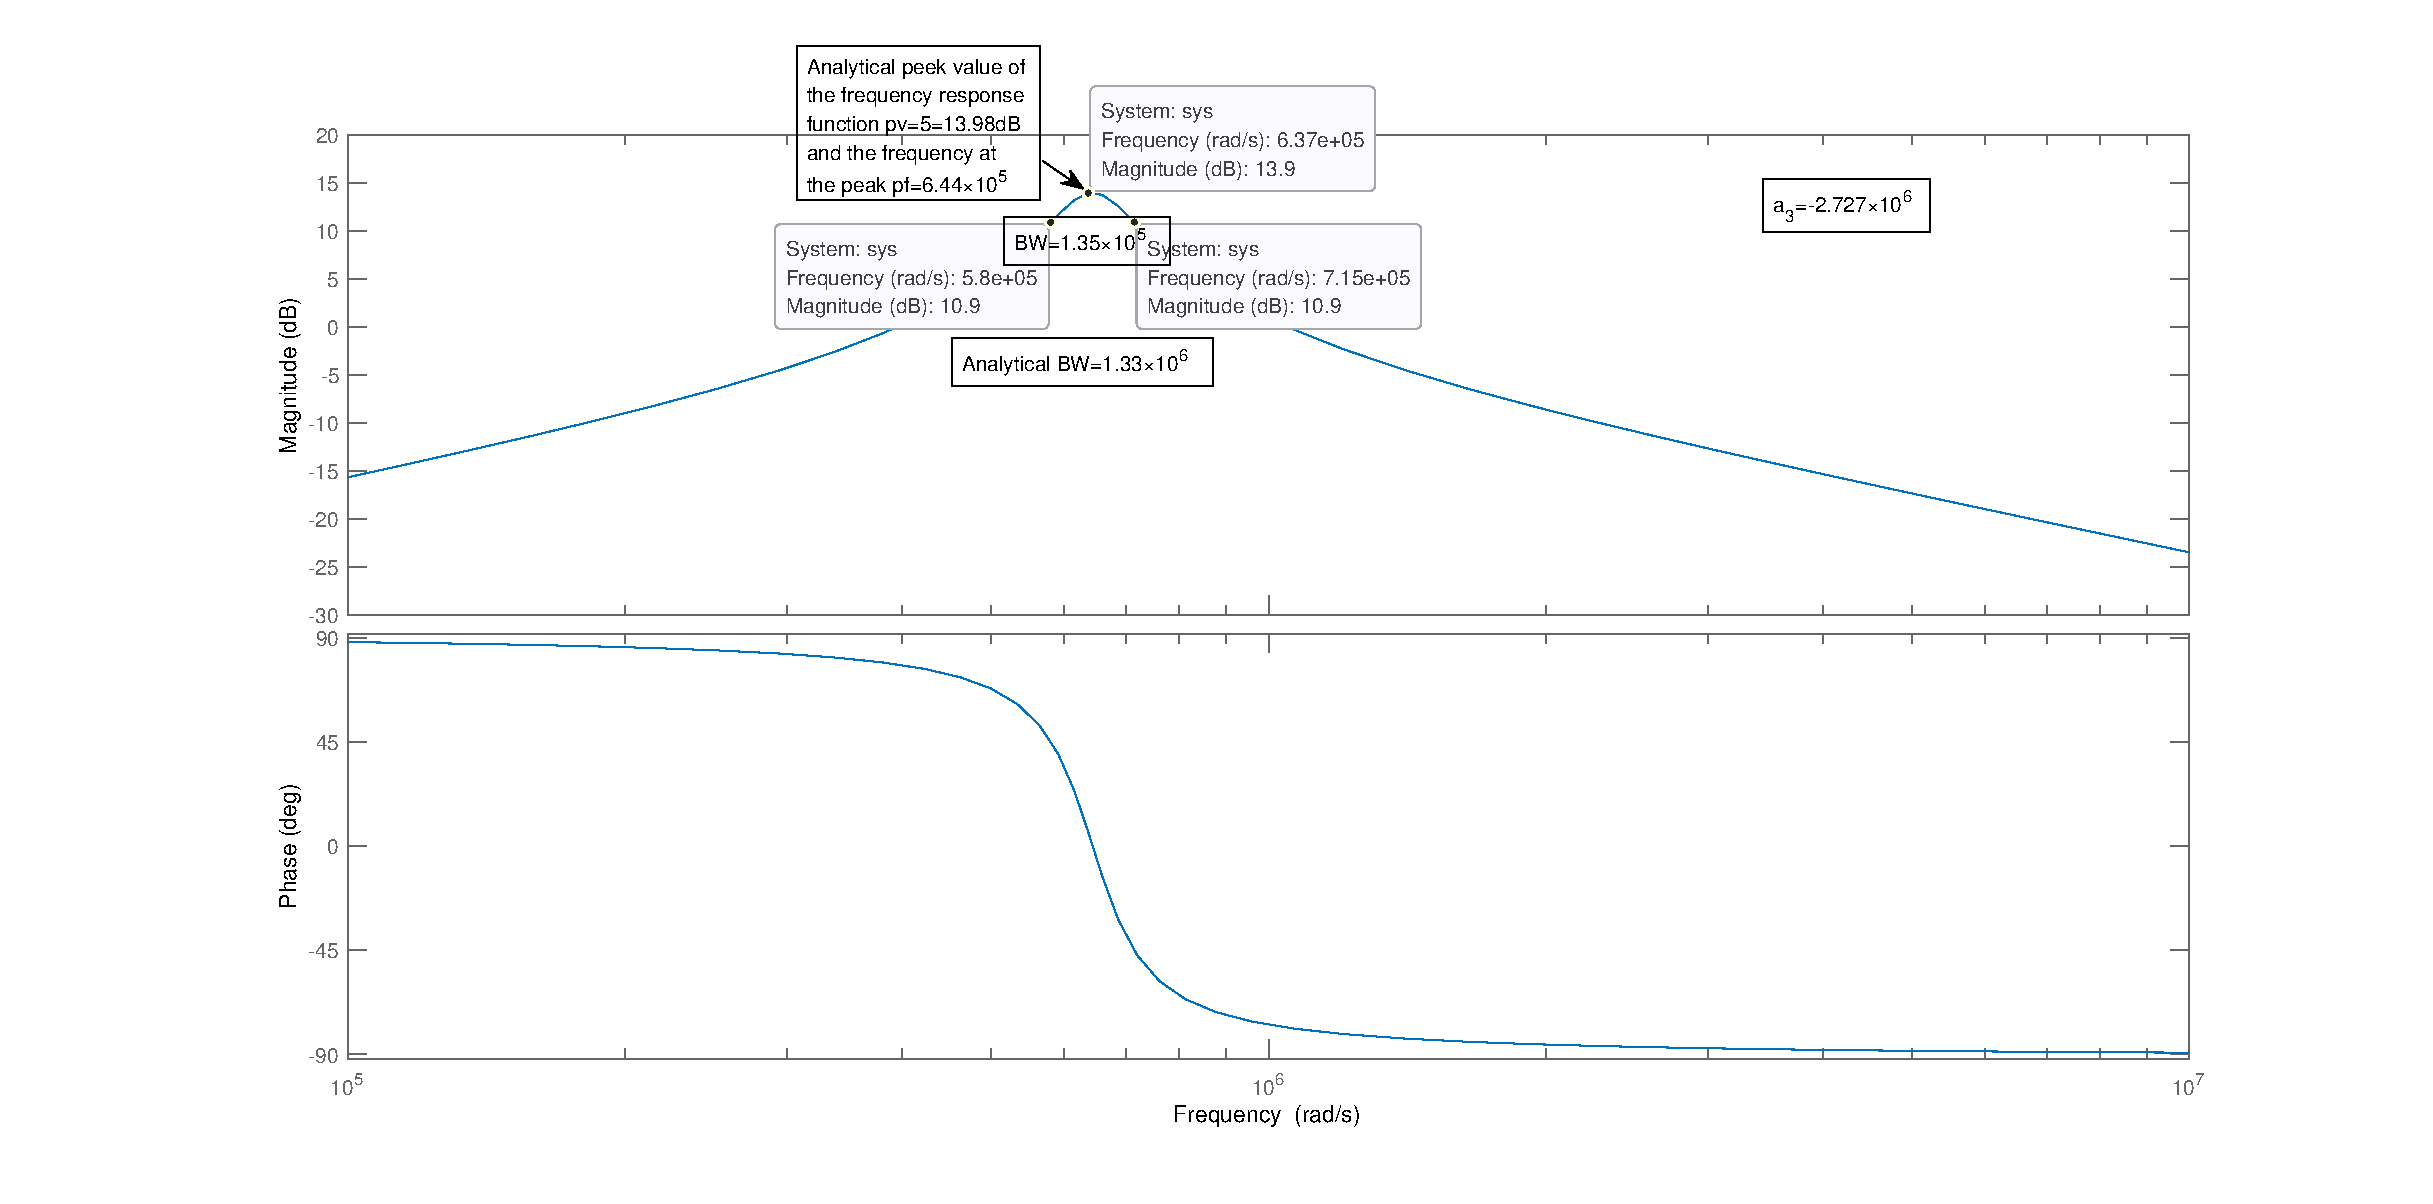
\includegraphics[width=1\textwidth]{3.2(c).eps}
    \end{center}
    \caption{3.2(c)}
\end{figure}
From the figure we can see that the analytical value of the peak value of the frequency response function and the frequency at the peak are very closed to the "exact" values read off my plot, however, the analytical value of $BW_{3dB}$ is not very closed to the "exact" value read off my plot.

MATLAB Code:
\lstinputlisting{P3_2_c.m}
\end{document}